\section{NodeControl}
\label{nodecontrol}

NodeControl is a small management application that runs on each validator node. It is in charge of carrying out simple update tasks.
It will listen to the local blockchain client via the HTTP RPC interface. If the local blockchain is not available it will fallback to the Incubed network to receive and verify update events \footnote{Incubed and this feature are not part of the MVP}.
The ethereum address of the validator account is used as a node identifier. NodeControl will only act on events directly directed to its assigned address.
This allows granular deployment of updates. \\

NodeControl will also track the local blockchain client to determine the current number of validators \footnote{MVP will have a fixed, configurable number of block to determine finality}. This is needed to determine finality of an update command.
The trigger process is shown in Fig. ~\ref{fig:nctrigger}.


\begin{figure}[ht]
	\centering
    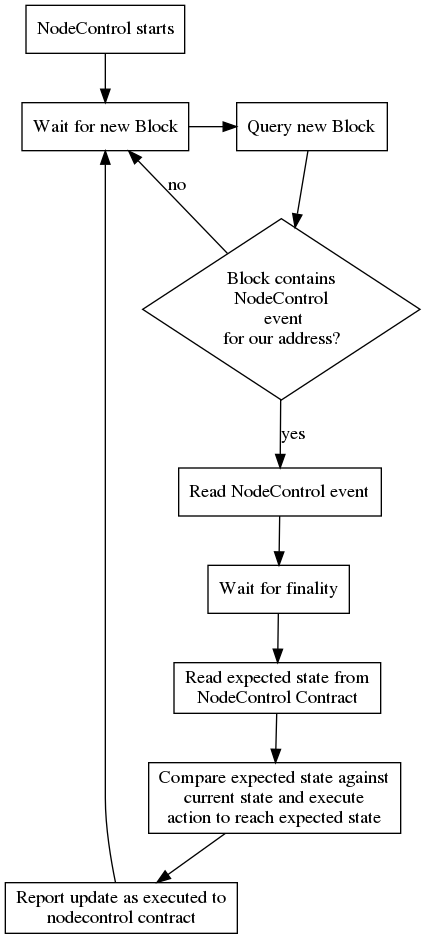
\includegraphics[height=0.65\textheight,keepaspectratio]{./images/nodecontrol.png}
	\caption{NodeControl Trigger Process}
	\label{fig:nctrigger}
\end{figure}

\newpage
\subsection{Interface to Contract}

This is an abstract definition of the Smartcontract interface between the NodeControl deamon and the accompanying contract on-chain.

\begin{itemize}

    \item \texttt{event UpdateAvailable(address targetValidator, unit eventId)} \\
    The contract has to emit this event once an update should be triggered on a node. If one would like to update multiple validators at once the event has to be send for each node individual.

    \item \texttt{function RetrieveUpdate(address targetValidator, unit eventId)} \\ \texttt{returns (uint command, byte[] payloadHash, string payload)} \\  
    NodeControl will call this function after finality has been reached to retrieve the actual command and payload. \\
    Command is an \texttt{uint} based on this map: \\
    \texttt{0 => updateParity} Will update the parity docker container. \\
    \texttt{1 => updateChainspec} Will update the chainspec file. \\
    \texttt{2 => enableSigner} Will restart Parity with signing enabled (payload and hash empty) \\
    \texttt{3 => disableSigner} Will restart Parity with signing disabled (payload and hash empty) \\

    The command code will also determine the meaning of the two remaining fields \texttt{payloadHash} and \texttt{payload}.

    \begin{itemize}
        \item \texttt{updateParity} \\
        \texttt{payloadHash} => The SHA256 Id of the docker image returned by \texttt{docker image inspect} \\
        \texttt{payload} => The dockerimage from dockerhub including tag (eg. \texttt{parity/parity:v2.2.5})

        \item \texttt{updateChainspec} \\
        \texttt{payloadHash} => The SHA256 hash of the downloaded file \\
        \texttt{payload} => HTTPS url to download the new chainspec 

    \end{itemize}
    
    \item \texttt{function ConfirmUpdate(unit eventId, boolean success)} \\
    After NodeControl carried out the update it will report back with a transaction calling this function. It will send a boolean if the update was successful or not. The transaction will be send from the validator account over HTTP RPC.

\end{itemize}
